%
% Surveys.tex
% Surveys
%
% R for Business Administration
%
% Copyright (C) 2016 Harris Kenny, Brandon DeGolier, Nate Lewis
%
% This document is licensed under the Creative Commons Attribution 4.0
% International Public License (CC BY-SA 4.0)
%

\section{Survey Recipients}
Surveys are a valuable way to learn stakeholders' perceptions of your 
organization's past, present, and future performance. Below are examples of 
survey recipients that may be relevant for your organization:

\begin{itemize}
 \item Advisors
 \item Channel Partners
 \item Customers
 \item Developers
 \item Educators
 \item Employees
 \item Journalists
 \item Investors
 \item Policymakers
 \item Suppliers
 \item Students
 \item Tradeshow Attendees
\end{itemize}

Let's try exercises using data that could be collected through surveys.

\section{Viewing Data}
The exercises in this section will use the "warpbreaks" dataset (The Number of 
Breaks in Yarn during Weaving) that is included with R. Load this data set into
 R following the instructions outlined in the Installation section of this work.

First, view the data by entering the following command in R Script or R 
Console:

\texttt{print(warpbreaks)}

This yields the following results:

\begin{figure}[htbp]
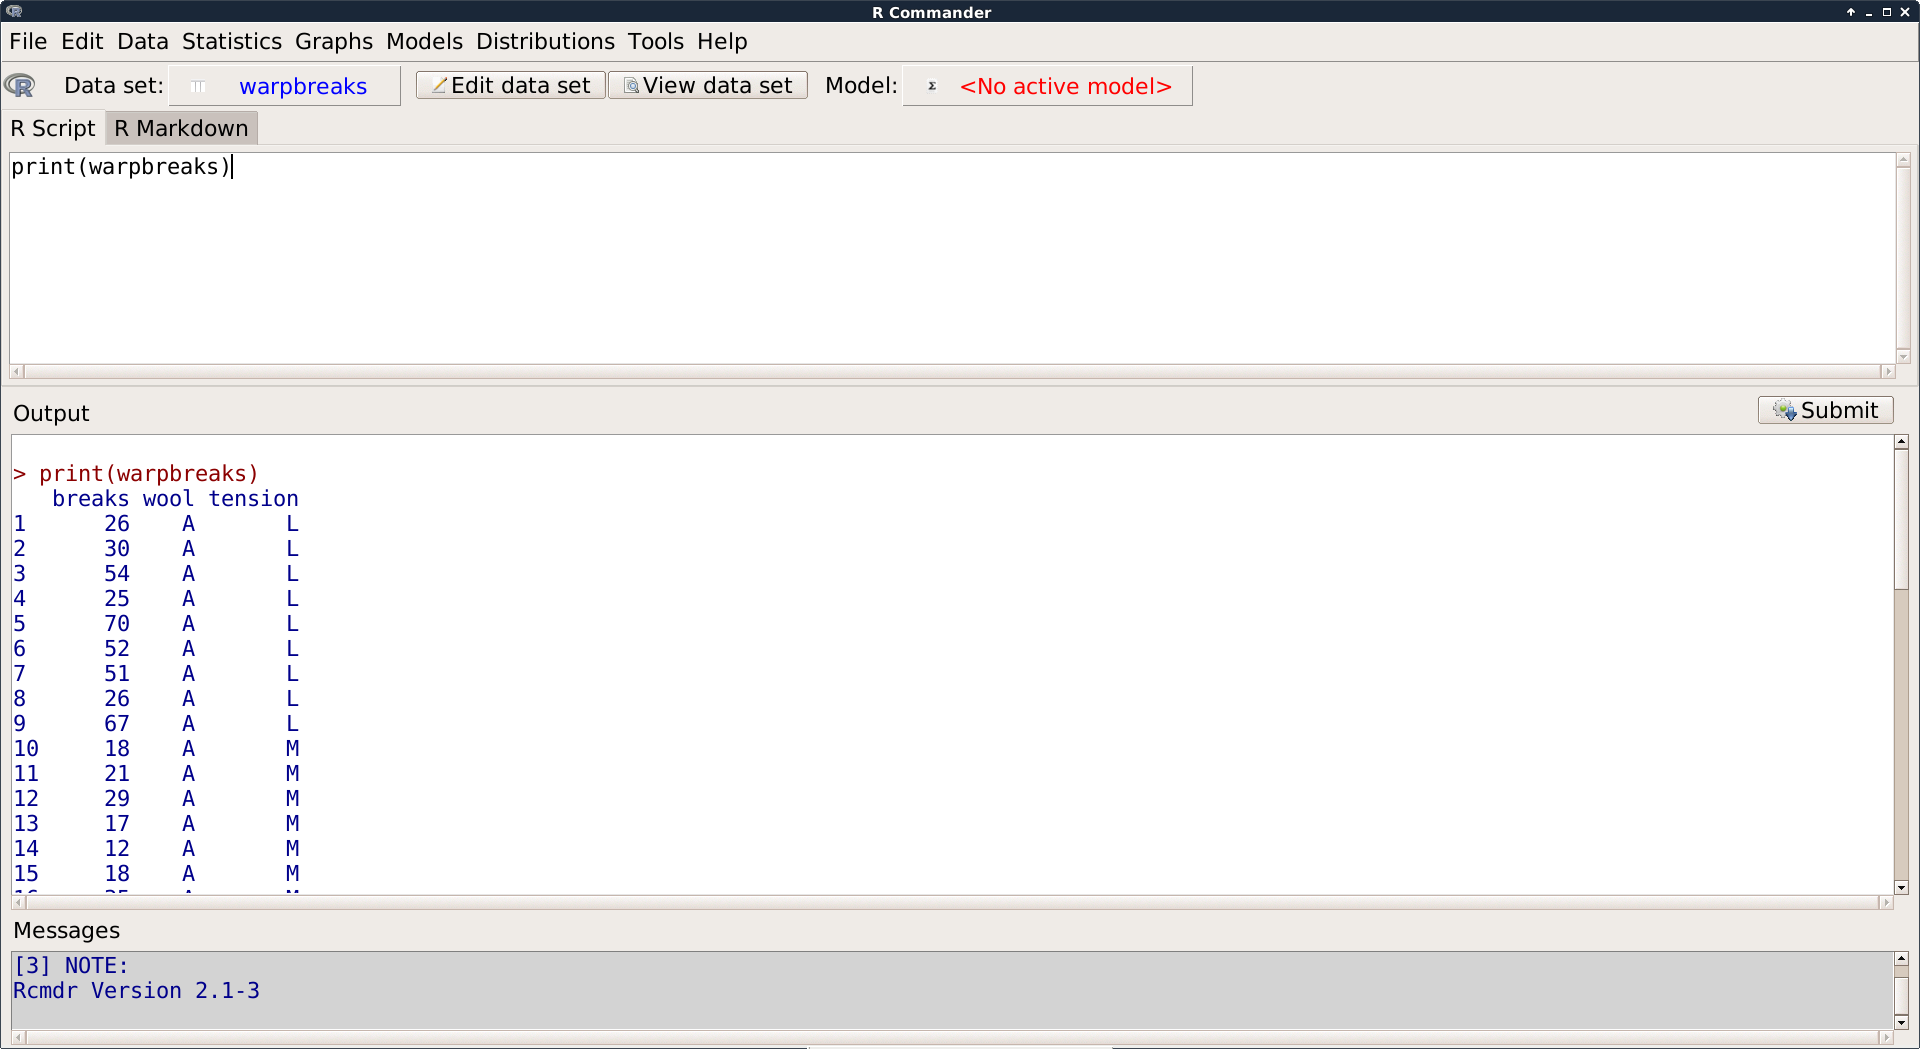
\includegraphics[keepaspectratio=true,height=1.10\textheight,width=1.00\textwidth,angle=0]{print_warpbreaks.png}
 \caption{warpbreaks dataset via R-Commander R Script}
 \label{fig:print_warpbreaks}
\end{figure}

Or, click View data set in R-Commander in the center of the user interface 
window.

This yields the following results:

\begin{figure}[htbp]
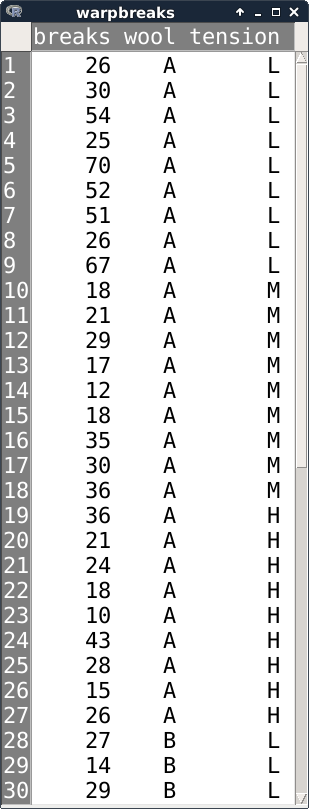
\includegraphics[keepaspectratio=true,height=1.10\textheight,width=1.00\textwidth,angle=0]{view-data-set_warpbreaks.png}
 \caption{warpbreaks dataset via R-Commander GUI}
 \label{fig:view-data-set_warpbreaks}
\end{figure}

This is a long dataset, let's understand the number we are dealing with by 
entering the following command:

\texttt{nrow(warpbreaks)}

This yields the following results:

[1] 54

Meaning there are 54 rows in the dataset, or 54 samples of yarn in 
consideration. Consider the context. The dataset includes three variables, 
shown as column headers\footnote{Beyond looking at column headers, recall that 
you can have R return the variable names by entering: names(warpbreaks)}:

\begin{enumerate}
 \item Breaks - The number of reported breaks for each sample of yarn.
 \item Wool - The type of wool for each sample of yarn. A categorial variable, 
 either A or B.
 \item Tension - The level of tension for each sample of yard. A categorical 
 variable, either L (low), M (medium), or H (high).
\end{enumerate}

Assume further that yarn breaking during weaving is problematic. In other 
words, the higher the number in the Breaks column for each row, the worse that 
sample of yarn has performed. 

\subsection{Averages and Quartiles}
Averages and quartiles are a basic way to capture a snapshot of the data you 
have collected. Recall there are two types of data (continuous and 
categorical), so R will generate two types of sets of summary statistics.

Calculate summary statistics by entering the following command:

\texttt{summary(warpbreaks)}

Or, select in R-Commander by going to Statistics > Summaries > Active Dataset. 
Either way, the result will be generated in the Output window in R-Commander.

This yields the following results:

\begin{figure}[htbp]
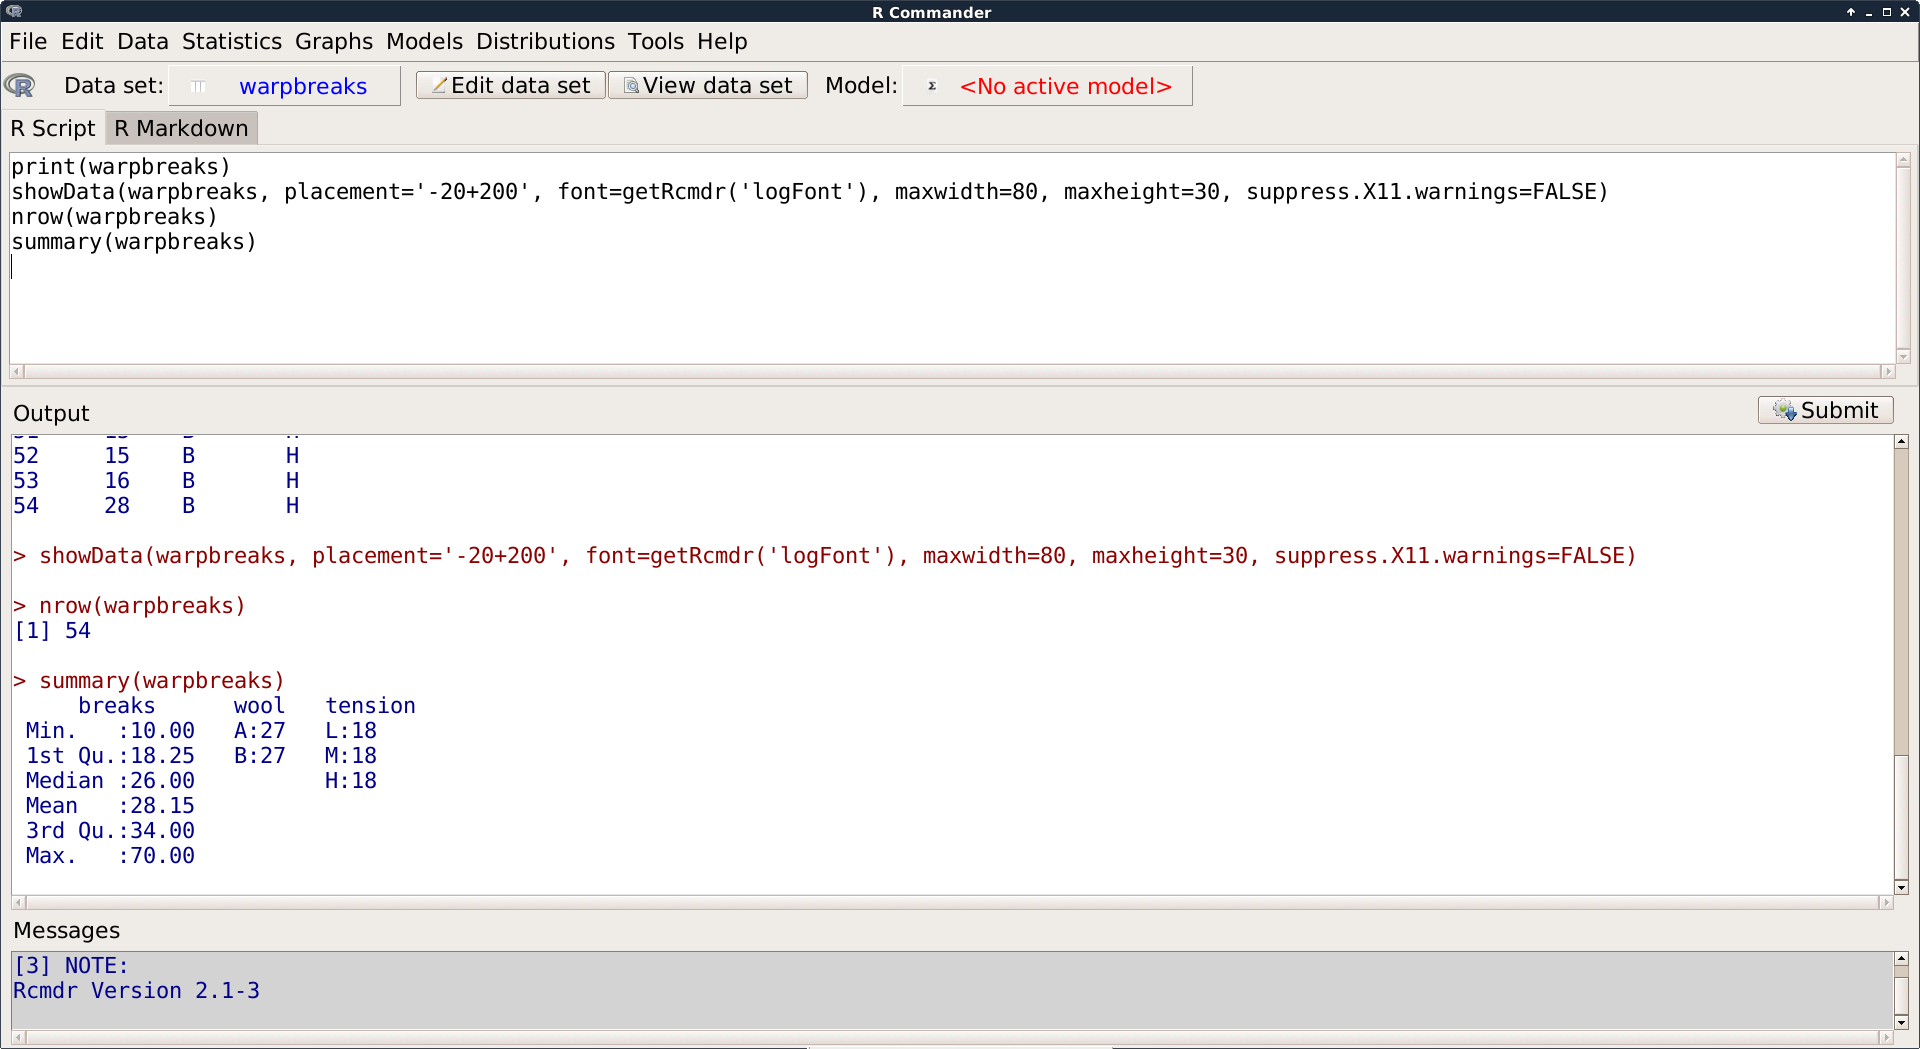
\includegraphics[keepaspectratio=true,height=1.10\textheight,width=1.00\textwidth,angle=0]{summary_warpbreaks.png}
 \caption{warpbreaks dataset summary via R-Commander R Script}
 \label{fig:summary_warpbreaks}
\end{figure}

What is the significance of these results? Let's break them down one-by-one:

\begin{itemize}
 \item \textbf{Min.} - The minimum data point in the dataset. For column 
 "breaks" this number is 10. In other words, of the surveyed samples of yarn, 
 the lowest number of observed breaks in the dataset is 10. Stated differently,
  the best performing yarn had 10 breaks.
 \item \textbf{1st Qu.} - The first quartile of data in the dataset. For column
  "breaks" this number is 18.25. In other words, of the surveyed samples of 
  yarn, the bottom quarter of yarn surveyed had 18.25 breaks.
 \item \textbf{Median} - The median datapoint in the dataset. For column 
 "breaks" this number is 26. In other words, of the surveyed samples of yarn, 
 the middle data point is 26. This is calculated by cross-secting the data to 
 the middle and selecting the single point, or adding the two middle points and
  dividing by two if the dataset has an even number. Median calculations are 
  especially valuable for datasets that have outliers that may be skewing mean 
  averages (more on this below).
 \item \textbf{Mean} - The mean datapoint for the dataset. For column "breaks" 
 this number is 28.15. This is calculated by summing all of the data points and
  dividing by the total number (or count) of data points. Mean is what most 
  people are referring to when they use the term average, and is the most 
  common form of average used.
 \item \textbf{3rd Qu.} - The third quartile of data in the dataset. For column
  "breaks" this number is 34. In other words, of the surveyed samples of yarn, 
  the top quarter of yarn surveyed had 34 breaks.
 \item \textbf{Max.} - The maximum data point in the dataset. For column 
 "breaks" this number is 70. In other words, of the surveyed samples of yarn, 
 the highest number of observed breaks in the dataset is 70. Stated 
 differently, the worst performing yarn had 70 breaks.
\end{itemize}

What else can we conclude from summary statistics of the "breaks" column? The 
mean is larger than the median, indicating a possible skew in the data towards 
the samples of yarn with higher numbers of breaks.

There are two other columns of summary statistics calculated by R: wool and 
tension. This provides a count summary of these categorical variables. Note 
that the dataset includes an even number of both types of wool (27 of both A 
and B). The dataset also includes an even number of all three levels of tension
 (18 Low, Medium, and High).

There is a third less common measure of average called mode\footnote{In R, mode
 is more importantly an object characteristic in indicating how the object is 
 stored in memory (e.g. as a number, as a character string, as a function).}, 
 the value that has the highest number of occurrences in the dataset. 
 Calculating mode takes several steps and is not outlined at this time.

% Fill this out later

\subsection{Pie Charts}
Pie charts are a common way to visualize data. Thanks to R-Commander, it is 
quick and easy to generate pie charts in R. The example below shows the three 
levels of tension, described above.

\begin{figure}[htbp]
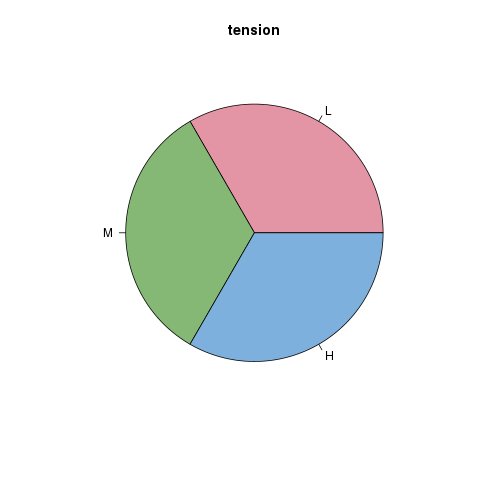
\includegraphics[keepaspectratio=true,height=1.10\textheight,width=1.00\textwidth,angle=0]{piechart_warpbreaks-tension.png}
 \caption{warpbreaks dataset tension pie chart via R-Commander GUI}
 \label{fig:summary_warpbreaks}
\end{figure}

\section{Generating Metadata from Open Responses}
% Section is incomplete, needs a screen shot to demonstrate how
It is possible to create metadata from open-ended responses in survey questions
 that you evaluate through statistical techniques.

For example, say a survey asked customers if there is anything your 
organization could do to better serve them in the future. Have someone from 
your organization review the responses and generate a list based on topics 
submitted by customers. 

Next, count each time on appears in the customer responses. This can be done 
manually or through a formula in spreadsheet software like LibreOffice Calc or 
Gnumeric.\footnote{Learn more about these projects at 
\texttt{https://www.libreoffice.org/} and \texttt{http://gnumeric.org/}} This 
new set of metadata can now be leveraged in proportion tests or other testing 
methods.